\section{Training}
\label{training_detail}

The SFT and preference-alignment data are processed in batches of 128, whereas RL batches contain 512 samples.  
We set the learning rate to $3\!\times\!10^{-4}$ for SFT and to $1\!\times\!10^{-5}$ for both S-DPO, together with a cosine decay scheduler. S-DPO is trained for a single epoch, and we fix $\beta=0.1$ and sample three negative items. For D$^{3}$, the interpolation coefficient $\alpha$ is chosen from $\{0.8, 0.9, 1.0\}$.  

For the SID generation stage of MiniOneRec, we utilise Qwen3-Embedding-4B as the LLM encoder to transform item titles and descriptions into their corresponding embeddings. The tokenizer is trained on 1 GPU with batch size of 20\,480. RQ-VAE is trained for 10\,000 epochs, with a learning rate of $1\!\times\!10^{-3}$. After embedding training, we use the Qwen2.5-Instruct series models as our backbone. The SFT stage is conducted on $8\times{}$NVIDIA H100 GPUs with a per-GPU batch size of 128 for up to ten epochs (early stopping, patience = 1). Finally, we perform two epochs of reinforcement learning with the same $\beta$. During rollout, we use beam search with a beam size of 16, generating 16 candidate trajectories for each input sample.

In the performance comparison with existing recommenders, all conventional recommender baselines are optimized with binary cross-entropy (BCE) loss and the Adam optimizer.  
The learning rate is selected from $\{1\!\times\!10^{-2}, 1\!\times\!10^{-3}, 1\!\times\!10^{-4}\}$, while the weight-decay coefficient is tuned within $\{1\!\times\!10^{-2}, 1\!\times\!10^{-3}, 1\!\times\!10^{-4}, 1\!\times\!10^{-5}, 1\!\times\!10^{-6}\}$.  
A mini-batch size of 1024 is used throughout.  
For TIGER, we adopt T5 \citep{T5} as the encoder–decoder backbone and use Qwen3-Embedding-4B to generate item embedding.  
Every LLM-based method, including ours, is built upon Qwen2.5-Instruct\citep{qwen2.5} to keep the computational footprint modest, and is trained with the AdamW optimizer.  

\section{Evaluation}
\label{results}
In this section, we first conduct a scaling study on two real-world benchmarks \citep{amazon}.
Then we report the empirical performance of \textbf{MiniOneRec}, and compare it against a selected set of baselines covering conventional sequential recommenders, SID-based generative models, and recent LLM-powered recommenders.
In addition, we recast the SID-based next-item prediction task as
recommendation rule discovery and show that MiniOneRec offers extra gains for cold-start users with scarce interactions and even for completely unseen domains.
We further conduct extensive ablation studies to pinpoint the components that most contribute to MiniOneRec’s effectiveness. 
Furthermore, we investigate how the general knowledge encoded in pre-trained LLM weights influences the performance of generative recommendation.
In summary, we study the following questions within this section:
\begin{itemize}[leftmargin=*]
    \item How does loss of MiniOneRec scale with different model size?
    
    \item How does MiniOneRec perform in comparison to other baseline methods?
    
    \item How does MiniOneRec perform under completely unseen domains?
    
    \item How do the designed components contribute to MiniOneRec's recommendation efficiency?

    \item How do the pre-trained weights of the LLM influence the performance of generative recommendation?
    % What is the impact of the designed components on the recommendation performance of MiniOneRec?

\end{itemize}

\subsection{Evaluation Setup}

\textbf{Datasets and Metrics.} 
We conduct extensive experiments on two real–world subsets of the Amazon Review corpus \citep{amazon} —\textit{Office} and \textit{Industrial}.  
% Among them, \textit{Office} and \textit{Industrial} are relatively small, each containing on average about 30\,000 user interaction sequences, whereas \textit{Books} is a large–scale dataset with more than 3\,million sequences.  
Following common practice, we adopt Hit Rate (HR@K) and Normalized Discounted Cumulative Gain (NDCG@K) to evaluate the top–$K$ recommendation accuracy. 


% Please add the following required packages to your document preamble:
% \usepackage{multirow}
\begin{table}[t]
\caption{Performance of MiniOneRec Compared to Traditional Methods, Generative Methods, and LLM-based Methods} 
\label{tab:overall}
\centering
\resizebox{0.86\textwidth}{!}{% 按比例缩放到页宽
\renewcommand{\arraystretch}{1.1}
\begin{tabular}{clllllll}
\hline
\multicolumn{1}{l}{Dateset}           & Methods    & HR@3   & NDCG@3 & HR@5   & NDCG@5 & HR@10  & NDCG@10 \\ \hline
\multirow{14}{*}{\textbf{Industrial}} & \multicolumn{7}{c}{\textbf{Traditional}}                          \\ \cline{2-8} 
                                      & GRU4Rec    & 0.0638 & 0.0542 & 0.0774 & 0.0598 & 0.0999 & 0.0669  \\
                                      & Caser      & 0.0618 & 0.0514 & 0.0717 & 0.0555 & 0.0942 & 0.0628  \\
                                      & SASRec     & 0.0790 & 0.0700 & 0.0909 & 0.0748 & 0.1088 & 0.0806  \\ \cline{2-8} 
                                      & \multicolumn{7}{c}{\textbf{Generative}}                           \\ \cline{2-8} 
                                      & HSTU       & 0.0927 & 0.0885 & 0.1037 & 0.0918 & 0.1163 & 0.0958  \\
                                      & TIGER      & 0.0852 & 0.0742 & 0.1010 & 0.0807 & 0.1321 & 0.0908  \\
                                      & LCRec      & 0.0915 & 0.0805 & 0.1057 & 0.0862 & 0.1332 & 0.0952  \\ \cline{2-8} 
                                      & \multicolumn{7}{c}{\textbf{LLM-based}}                            \\ \cline{2-8} 
                                      & BIGRec     & 0.0931 & 0.0841 & 0.1092 & 0.0907 & 0.1370 & 0.0997  \\
                                      & D$^3$         & 0.1024 & \uline{0.0991} & 0.1213 & 0.0989 & 0.1500 & \uline{0.1082}  \\
                                      & S-DPO      & \uline{0.1032} & 0.0906 & \uline{0.1238} & \uline{0.0991} & \uline{0.1524} & \uline{0.1082}  \\ \cline{2-8} 
                                      & \multicolumn{7}{c}{\textbf{Ours}}                                 \\ \cline{2-8} 
                                      & MiniOneRec      & \textbf{0.1125} & \textbf{0.0988} & \textbf{0.1259} & \textbf{0.1046} & \textbf{0.1546} & \textbf{0.1139}  \\
                                      \hline
\multirow{14}{*}{\textbf{Office}}     & \multicolumn{7}{c}{\textbf{Traditional}}                          \\ \cline{2-8} 
                                      & GRU4Rec    & 0.0629 & 0.0528 & 0.0789 & 0.0595 & 0.1019 & 0.0669  \\
                                      & Caser      & 0.0748 & 0.0615 & 0.0865 & 0.0664 & 0.1093 & 0.0737  \\
                                      & SASRec     & 0.0861 & 0.0769 & 0.0949 & 0.0805 & 0.1120 & 0.0858  \\ \cline{2-8} 
                                      & \multicolumn{7}{c}{\textbf{Generative}}                           \\ \cline{2-8} 
                                      & HSTU       & 0.1134 & 0.1031 & 0.1252 & 0.1079 & 0.1400 & 0.1126  \\
                                      & TIGER      & 0.0986 & 0.0852 & 0.1163 & 0.0960 & 0.1408 & 0.1002  \\
                                      & LCRec      & 0.0921 & 0.0807 &    0.1048 & 0.0859 & 0.1237 & 0.0920  \\ \cline{2-8} 
                                      & \multicolumn{7}{c}{\textbf{LLM-based}}                            \\ \cline{2-8} 
                                      & BIGRec     & 0.1069 & 0.0961 & 0.1204 & 0.1017 & 0.1434 & 0.1091  \\
                                      & D$^{3}$         & \uline{0.1204} & \uline{0.1055} & \uline{0.1406} & \uline{0.1139} & \textbf{0.1634} & 0.1213  \\
                                      & S-DPO      & 0.1169 & 0.1033 & 0.1356 & 0.1110 & \uline{0.1587} & \textbf{0.1255}  \\ \cline{2-8} 
                                      & \multicolumn{7}{c}{\textbf{Ours}}                                 \\ \cline{2-8} 
                                      & MiniOneRec      & \textbf{0.1217} & \textbf{0.1088} & \textbf{0.1420} & \textbf{0.1172} & \textbf{0.1634} & \uline{0.1242}  \\
                                      \hline
\end{tabular}
}
\end{table}

\subsection{Scaling}
We demonstrate the scaling capabilities of MiniOneRec, where the convergence loss decrease consistently as the model size increases. 
As Fig. \ref{fig:scaling} shows, under the generative recommendation paradigm, there is a clear correlation between model size and loss. As the LLM scale increases, the convergence loss continues to decrease. Furthermore, Figure. \ref{fig:scaling_eval_loss} tracks the evaluation loss on the SFT training set, recorded every 0.5 epoch. It is evident that models with larger parameter counts maintain lower evaluation losses throughout nearly the entire training process and converge more rapidly.
Such a superior scaling effect demonstrates the potential of generative recommenders as the next-generation recommendation models.

% \subsection{Performance Comparison (RQ1)}
\subsection{Performance Comparison}

\textbf{Experimental Settings}.
All conventional recommender baselines are optimized with binary cross-entropy (BCE) loss and the Adam optimizer.  
The learning rate is selected from $\{1\!\times\!10^{-2}, 1\!\times\!10^{-3}, 1\!\times\!10^{-4}\}$, while the weight-decay coefficient is tuned within $\{1\!\times\!10^{-2}, 1\!\times\!10^{-3}, 1\!\times\!10^{-4}, 1\!\times\!10^{-5}, 1\!\times\!10^{-6}\}$.  
A mini-batch size of 1024 is used throughout.  
For TIGER, we adopt T5 \citep{T5} as the encoder–decoder backbone and use Qwen3-Embedding-4B to generate item embedding.  
Every LLM-based method, including ours, is built upon Qwen2.5-Instruct-0.5B \citep{qwen2.5} to keep the computational footprint modest, and is trained with the AdamW optimizer.  
The SFT and preference-alignment data are processed in batches of 128, whereas RL batches contain 512 samples.  
We set the learning rate to $3\!\times\!10^{-4}$ for SFT and to $1\!\times\!10^{-5}$ for both S-DPO and MiniOneRec, together with a cosine decay scheduler.  
SFT runs for ten epochs with early stopping (patience = 1). S-DPO is trained for a single epoch, and we fix $\beta=0.1$ and sample three negative items. For D$^{3}$, the interpolation coefficient $\alpha$ is chosen from $\{0.8, 0.9, 1.0\}$.  
\begin{wrapfigure}[14]{r}{0.48\columnwidth}   % 14 可根据需要微调
    \centering
    \vspace{12pt}                             % 细调上边距
    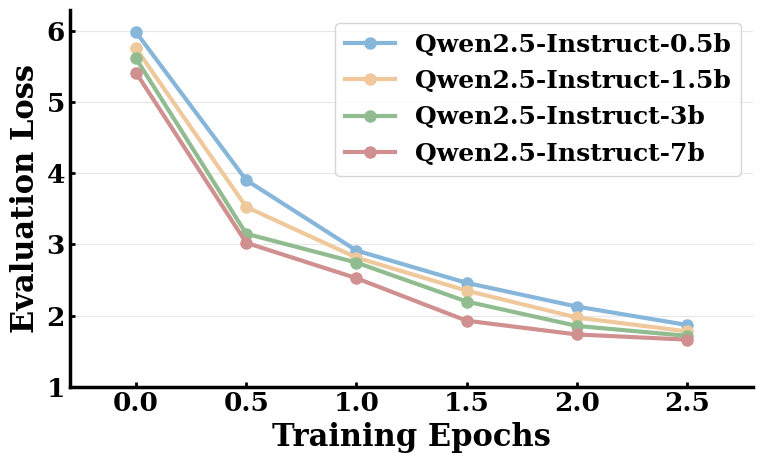
\includegraphics[width=\linewidth]{figures/scaling_eval_loss.png}
    \vspace{-12pt}                             % 细调下边距
    \caption{Evaluation loss vs.\ SFT training epoch}
    \label{fig:scaling_eval_loss}
\end{wrapfigure}

\textbf{Baselines.} 
Our baselines contain three categories: (1) Traditional recommendation models, including GRU4Rec \citep{GRU4Rec}, Caser \citep{Caser}, SASRec \citep{SASRec}; (2) Generative recommendation models: HSTU \citep{HSTU}, TIGER \citep{TIGER}, LC-Rec \citep{LCRec}; (3) LLM-based recommendation models, including BigRec \citep{BIGRec}, D$^3$ \citep{D3}, S-DPO \citep{sdpo}.

We conduct a comprehensive evaluation of \textsc{MiniOneRec} on two benchmark datasets—Industrial and Office; the results are summarized in Table \ref{tab:overall}. 
Two major observations emerge:

\begin{itemize}[leftmargin=*]
    \item \textbf{Utility of LLM World Knowledge.} LLM-based recommenders such as BIGRec and D$^3$ markedly outperform classical paradigms like GRU4Rec and Caser, confirming that injecting the broad world knowledge encoded in LLMs can substantially boost recommendation quality.
    \item \textbf{Effectiveness of MiniOneRec.} By incorporating fine-grained SID information into the RL loop and aligning the entire generation trajectory with the task objective, MiniOneRec delivers a marked improvement over existing generative recommendation approaches, achieving consistent gains across all evaluated metrics. When contrasted with the current SOTA LLM-based recommendation paradigms, it continues to outperform the strongest baselines. Moreover, by operating in the compact SID space rather than on verbose textual titles, MiniOneRec requires substantially fewer context tokens and yields faster inference, translating into lower latency and smaller memory footprints at serving time.
\end{itemize}

% \begin{table}[t]
% \caption{Performance of MiniOneRec and its variants on completely unseen recommendation domains} 
% \label{tab:ood}
% \resizebox{\textwidth}{!}{% 按比例缩放到页宽
% \begin{tabular}{clllllll}
% \hline
% \multicolumn{1}{l}{Dataset}      & Method                    & HR@3            & NDCG@3          & HR@5            & NDCG@5          & HR@10           & NDCG@10         \\ \hline
% \multirow{5}{*}{\textbf{Office}} & GRU4Rec                   & 0.0629          & 0.0528          & 0.0789          & 0.0595          & 0.1019          & 0.0669          \\
%                                  & Qwen-Text               & 0.0031          & 0.0021          & 0.0044          & 0.0026          & 0.0057          & 0.0030          \\
%                                  & Qwen-SID                 & 0.0300          & 0.0214          & 0.0456          & 0.0282          & 0.0733          & 0.0373          \\
%                                  % & MiniOneRec & 0.0068          & 0.0056          & 0.0080          & 0.0061          & 0.0138          & 0.0080          \\
%                                  & MiniOneRec-w/o SFT     & \uline{0.0553} & \uline{0.0433} & \uline{0.0691} & \uline{0.0489} & \uline{0.0892} & \uline{0.0553} \\ \hline
% \end{tabular}
% }
% \end{table}

% \subsection{Unseen-Domain Performance Evaluation (RQ2)}
\subsection{Transferability}
\label{subsec: Transferability}

To assess MiniOneRec's transferability to out-of-distribution (OOD) data, we conduct an unseen-domain study termed \emph{SID pattern discovery}. 
Specifically, the model is trained on the source domain Industrial and evaluated on a completely unseen target domain Office. Given that prior studies have shown SFT can overfit to the training domain and degrade OOD performance \citep{RLvsSFT, RLReallyLearn, SFT-then-RL, RevisitingRL}, we introduce an RL-only variant, MiniOneRec-w/ RL, specifically to provide a version focused on OOD generalization. We benchmark three systems:  
(1) GRU4Rec, trained and tested on Office.
(2) Qwen-Text, which encodes the user’s interaction history as plain text and predicts the next item in textual form;  
(3) Qwen-SID, which represents the same history as a sequence of SIDs and predicts the next SID;  
(4) MiniOneRec-w/ RL, which is trained solely with RL on Industrial and is tested on Office without SFT.  

As reported in Table~\ref{tab:ood}, Qwen-Text performs rather poorly, whereas Qwen-SID is markedly better, demonstrating that the structured SID space is easier for a language model to exploit. 
Although MiniOneRec-w/ RL lags behind the full MiniOneRec on in-domain metrics, its RL-only optimization offers strong transferability, yielding competitive accuracy on the unseen Office catalogue surprisingly.
Despite the substantial domain shift and the possible semantic mismatch among SIDs, MiniOneRec can still discover transferable interaction patterns and produce high-quality recommendations for a brand-new catalogue, highlighting the encouraging unseen-domain potential of our framework.



% \subsection{Training and Inference Cost Comparison (RQ3)}

% To comprehensively evaluate the resource efficiency of MiniOneRec, we compare its training cost with that of SOTA LLM-based recommenders fine-tuned via SFT. Specifically, we report GPU-hours to provide a more granular view of the overall expenditure.
% We carry out the cost analysis on the industry scale Books dataset, as illustrated in Figure x. Although MiniOneRec still adopts a two-stage pipeline of SFT followed by RL, its inputs and outputs are encoded as SID sequences, whose token count is an order of magnitude smaller than the free form text used by previous LLM-based recommenders. On the Books corpus we reserve only a small held out split for the RL phase, so the additional computation remains marginal. Overall, MiniOneRec delivers marked performance gains without inflating the training budget and simultaneously preserves the multi-modal SID interface.
% Beyond training cost, we measure online efficiency by reporting average latency per recommendation request. Owing to its compact SID representation, MiniOneRec requires substantially fewer decoding steps during inference than other LLM-based baselines. As displayed in Figure x, MiniOneRec cuts inference latency by 70\%, while using the same GPU batch size. These results indicate that MiniOneRec is not only cost-effective during training but also practical for real-time serving scenarios.

% \subsection{Ablation Study (RQ3)}
\subsection{Ablation Study}

To validate the effectiveness of each component in the MiniOneRec framework, we compare it with the following alternative approaches. 

\subsubsection{Aligning Strategy}

\begin{table}[t]
\caption{Performance of MiniOneRec and its variants on completely unseen recommendation domains} 
\label{tab:ood}
\resizebox{\textwidth}{!}{% 按比例缩放到页宽
\begin{tabular}{clllllll}
\hline
\multicolumn{1}{l}{Dataset}      & Method                    & HR@3            & NDCG@3          & HR@5            & NDCG@5          & HR@10           & NDCG@10         \\ \hline
\multirow{5}{*}{\textbf{Office}} & GRU4Rec                   & 0.0629          & 0.0528          & 0.0789          & 0.0595          & 0.1019          & 0.0669          \\
                                 & Qwen-Text               & 0.0031          & 0.0021          & 0.0044          & 0.0026          & 0.0057          & 0.0030          \\
                                 & Qwen-SID                 & 0.0300          & 0.0214          & 0.0456          & 0.0282          & 0.0733          & 0.0373          \\
                                 % & MiniOneRec & 0.0068          & 0.0056          & 0.0080          & 0.0061          & 0.0138          & 0.0080          \\
                                 & MiniOneRec-w/o SFT     & \uline{0.0553} & \uline{0.0433} & \uline{0.0691} & \uline{0.0489} & \uline{0.0892} & \uline{0.0553} \\ \hline
\end{tabular}
}
\end{table}

We benchmark the full model against three carefully designed variants:
(1) \textsc{MiniOneRec}--\textsc{w/o~Align}: A pure \textit{SID$\rightarrow$SID} paradigm: the input consists of SID-organized user histories, and the target is the SID of the next item. No cross-modal alignment is applied in either stage. 
(2) \textsc{MiniOneRec}--\textsc{w/~SFTAlign}: Alignment tasks are used only during the SFT stage, whereas the RL stage is trained on SID-only data.
(3) \textsc{MiniOneRec}--\textsc{w/~RLAlign}: The SFT stage relies on SID-only supervision, while alignment tasks are introduced solely in the RL stage.
% \begin{itemize}[leftmargin=*]
%     \item \textsc{MiniOneRec}--\textsc{w/o~Align.} A pure \textit{SID$\rightarrow$SID} paradigm: the input consists of SID-organized user histories, and the target is the SID of the next item. No cross-modal alignment is applied in either stage. 
%     \item \textsc{MiniOneRec}--\textsc{w/~SFTAlign.} Alignment tasks are used only during the SFT stage, whereas the RL stage is trained on SID-only data. 
%     \item \textsc{MiniOneRec}--\textsc{w/~RLAlign.} The SFT stage relies on SID-only supervision, while alignment tasks are introduced solely in the RL stage.
% \end{itemize}

As illustrated in Figure \ref{fig:ab1}, the full MiniOneRec with full-process SID alignment achieves the best results across all metrics. The \textsc{MiniOneRec}--\textsc{w/o~Align} variant performs the worst, underscoring the importance of grounding world knowledge when generating SIDs. Notably, although introducing the alignment objective directly in the RL stage is highly challenging for an LLM that has not been pre-conditioned by SFT, \textsc{MiniOneRec}--\textsc{w/~RLAlign} still yields a non-trivial gain. We attribute this improvement to our SID-Guided RL scheme, which offers the agent additional opportunities to obtain valid rewards on hard examples that conventional RL would likely miss.

\subsubsection{Sampling Strategy}

We contrast the full model with three variants that differ only in the way trajectories are collected:
(1) \textsc{MiniOneRec}--\textsc{Common} that uses a conventional top-$k$ decoding scheme to generate the required number of trajectories.
(2) \textsc{MiniOneRec}--\textsc{Dynamic}, which implements our dynamic sampler that first produces $\tfrac32$ times the target trajectory budget and then keeps as many distinct items as possible for RL optimization.
% \begin{itemize}[leftmargin=*]
%     \item \textsc{MiniOneRec}--\textsc{Common.} 
%     Uses a conventional top-$k$ decoding scheme to generate the required number of trajectories.
%     \item \textsc{MiniOneRec}--\textsc{Dynamic.} 
%     Implements our dynamic sampler that first produces $\tfrac32$ times the target trajectory budget and then keeps as many distinct items as possible for RL optimization.
%     \item \textsc{MiniOneRec}--\textsc{w/~Beam.} 
%     Retains only beam search; no SID-prefix guidance is applied, and all examples maintain their original difficulty level.
% \end{itemize}

As Figure \ref{fig:ab2} illustrates, the full MiniOneRec achieves the best overall performance, and attains higher accuracy than \textsc{MiniOneRec}--\textsc{Dynamic} while requiring only two-thirds of its sampling budget, showing that beam search is a more cost-effective backbone.

\subsubsection{Reward Design}
% Beyond binary correctness, recommendation scenarios naturally allow the use of richer dense signals that may further enhance alignment. 
% \tjf{For further exploration}, we investigate two recommendation-specific dense rewards: 
% \begin{itemize}[leftmargin=*]
%     \item \textbf{Semantic reward.} This reward measures the semantic similarity between the generated item and the target item, encouraging LLMs to capture semantic relatedness between items. 
%     \item \textbf{Collaborative reward.} To inject collaborative signals, each generated item is assigned the corresponding logit output by a traditional recommender system, reflecting collaborative filtering knowledge from historical user-item interactions.
% \end{itemize}
% These dense rewards offer a complementary perspective to binary correctness and allow us to examine whether richer supervision can 
% substitute rule-based signals in RLVR for recommendation.

Three variants are compared:
(1) \textsc{MiniOneRec}--\textsc{w/~acc} that uses the accuracy reward only;
(2) \textsc{MiniOneRec}--\textsc{w/~Collaborative} that uses SASRec to assign each item during sampling a corresponding logit output as its prediction score, thereby injecting collaborative reward information.

% \begin{itemize}[leftmargin=*]
%    \item \textsc{MiniOneRec}--\textsc{w/~acc.} 
%    Uses the accuracy reward only.
%    \item \textsc{MiniOneRec}--\textsc{w/o~SID.} Removes the SID-level reward for hard cases; the LLM is optimized with the accuracy plus rank rewards.
%    \item \textsc{MiniOneRec}--\textsc{w/~SIDAll.} 
%    Applies the SID-level reward to every training sample rather than restricting it to difficult ones.
% \end{itemize}
As shown in the Figure \ref{fig:ab3}, the full MiniOneRec achieves the best overall performance. To be noticed, injecting the collaborative reward information into the RL process instead led to significant degradation. We hypothesize that, this stems from reward hacking: as recommendation accuracy declines, the reward continues to increase, revealing a misalignment between this collaborative reward signal and the true objective.

\begin{figure*}[t]
  \centering
  \begin{subfigure}[t]{0.28\textwidth}
    \centering
    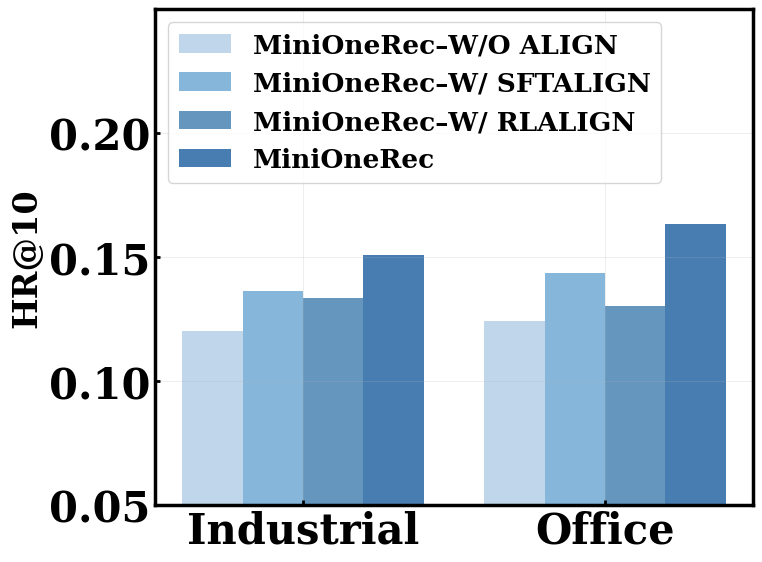
\includegraphics[width=\textwidth]{figures/ab1.png}
    \caption{Aligning Strategy.}
    \label{fig:ab1}
\end{subfigure}\hspace{2mm}
\begin{subfigure}[t]{0.28\textwidth}
    \centering
        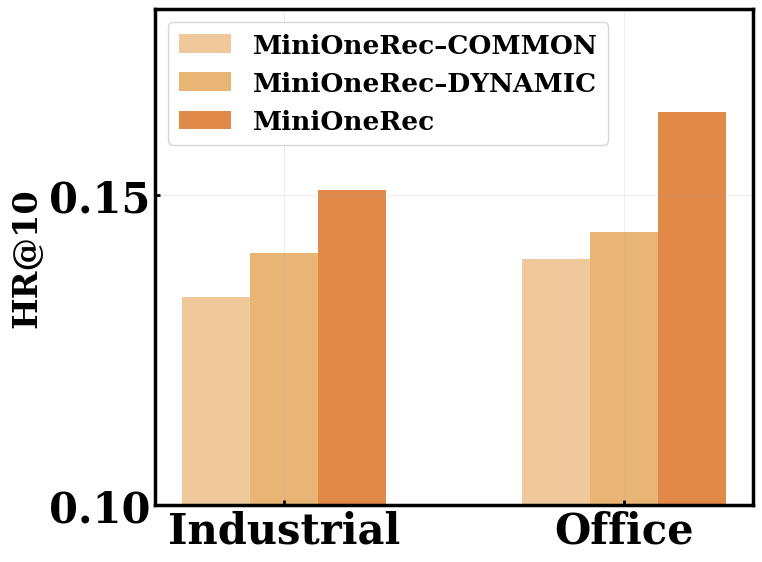
\includegraphics[width=\textwidth]{figures/ab2.png}
    \caption{Sampling Strategy.}
    \label{fig:ab2}
\end{subfigure}
\centering
  \begin{subfigure}[t]{0.28\textwidth}
    \centering
    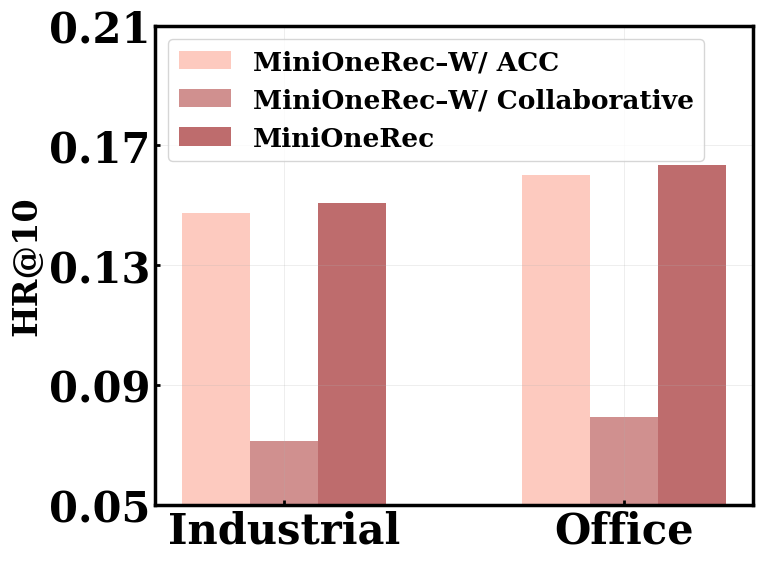
\includegraphics[width=\textwidth]{figures/ab3.png}
    \caption{Reward Design.}
    \label{fig:ab3}
\end{subfigure}\hspace{2mm}
  \caption{Study on the effectiveness of MiniOneRec’s individual components.
Figure \ref{fig:ab1} examines model performance under different alignment strategies;
Figure \ref{fig:ab2} investigates various sampling strategies;
Figure \ref{fig:ab3} evaluates the impact of alternative reward designs.}
  \label{fig:ablation}
    \vspace{-10pt}
\end{figure*}



% Please add the following required packages to your document preamble:
% \usepackage{multirow}
\begin{table}[]
\caption{Performance of MiniOneRec initialized with pre-trained weights versus random initialization across two domains} 
\label{tab:pretrain-impact}
\resizebox{\textwidth}{!}{% 按比例缩放到页宽
\begin{tabular}{clllllll}
\hline
\multicolumn{1}{l}{Dateset}          & Methods            & HR@3            & NDCG@3          & HR@5            & NDCG@5          & HR@10           & NDCG@10         \\ \hline
\multirow{2}{*}{\textbf{Industrial}} & MiniOneRec-scratch & 0.0757          & 0.0672          & 0.0891          & 0.0726          & 0.1134          & 0.0804          \\
                                     & MiniOneRec         & \textbf{0.1125} & \textbf{0.0988} & \textbf{0.1259} & \textbf{0.1046} & \textbf{0.1546} & \textbf{0.1139} \\ \hline
\multirow{2}{*}{\textbf{Office}}     & MiniOneRec-scratch & 0.0959          & 0.0855          & 0.1057          & 0.0896          & 0.1196          & 0.0941          \\
                                     & MiniOneRec         & \textbf{0.1217} & \textbf{0.1088} & \textbf{0.1420} & \textbf{0.1172} & \textbf{0.1634} & \textbf{0.1242} \\ \hline
\end{tabular}
}
\end{table}


\subsection{Pre-trained LLM Impact}
\label{llmmatter}
To isolate the impact pre-trained LLM on generative recommendation, we instantiate two variants of MiniOneRec: one initialized from a general-purpose pre-trained LLM and the other trained from scratch with random weights. As shown in Table \ref{tab:pretrain-impact}, Experiments on two benchmark datasets reveal a consistent pattern: the model that starts from pre-trained weights significantly outperforms its randomly initialized counterpart. We conjecture that (i) the general reasoning ability acquired during large-scale language pre-training allows the model to cast the next-SID prediction task as a problem of pattern discovery, as discussed in Section~\ref{subsec: Transferability}, and (ii) the factual knowledge already encoded in the LLM offers a head start in understanding the real-world semantics behind each SID, part of which can be transferred to the recommendation domain.